\section{Introduction}
Midsurface is an idealized representation of a thin-wall part, used mainly for creating shell elements in CAE meshing process. To be truly effective, Midsurface needs to mimic the original part in both, geometrical and topological sense. Geometrically, the shape of the Midsurface should be such that it lies in the middle (at half the thickness) of the part. By topological sense, it is expected that it should have connectivity between sub-shapes of the original part, reflected in the Midsurface as well. It would be easier to verify the output-Midsurface, using sound theoretical topological invariant(s), so that one does not have to resort to manual inspection for checking correctness of the output. 

Many thin-wall parts are from Sheet Metal domain. 
%There are specialized Sheet Metal modelers and also the specialized Sheet Metal Environment-workbench built in general CAD modeler for modeling them.  
These parts are peculiar, in both, geometric as well as topological ways:
\begin{itemize}
[noitemsep,topsep=2pt,parsep=2pt,partopsep=2pt,leftmargin=*]
\item \textbf{Constant thickness}: As Sheet Metal parts are made up of constant guage blank, thickness of all sub-shapes is constant. 
\item \textbf{Principal-Capping}: There are principal faces, which are part of the original blank and there are capping faces which are the side-thickness faces.

%\begin{wrapfigure}{l}{0.4\linewidth}
\begin{center} 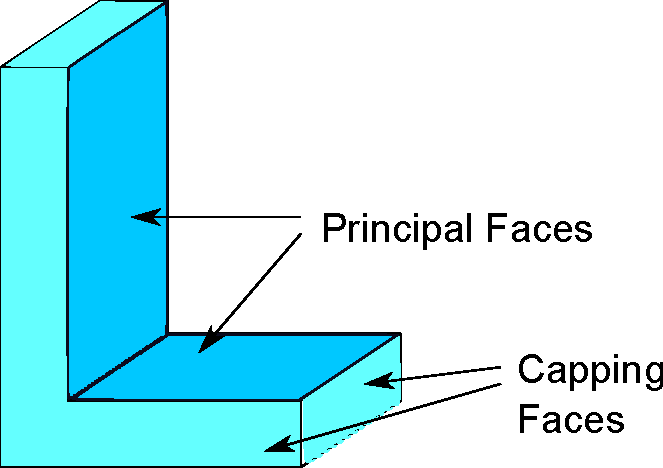
\includegraphics[width=0.34\linewidth]{../Common/images/PrincipalCappingL.pdf}
\end{center}
%\caption{Example: Principal and Capping Faces}
%\label{fig_principalcapping}
%\end{wrapfigure} 

\item \textbf{Absences}: There are no blind holes but only through holes, if any. There are no degenerate capping-thickness faces (like 'Wedge').
\begin{center} 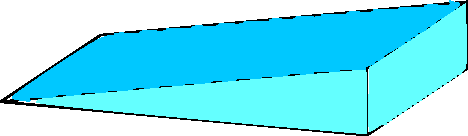
\includegraphics[width=0.34\linewidth]{../Common/images/WedgeTopology.pdf}
\end{center}
\item \textbf{Special Non-manifold}: Non manifoldness of their Midsurface is not in terms of edge-edge or vertex-vertex touching or partitions. Its due to its {\em surface} nature.
\item \textbf{Cavities}: There are no embedded volumes-cavities.
\end{itemize}


Many of the commercial Sheet Metal CAD modelers are based on data-structure called Boundary Representation.

\section{Boundary Representation (Brep)}
Brep is composed of two parts: topology and geometry. Topological elements are, {\em shells, faces, edges, vertices} etc. They are in the descending order of the topological dimensionality.  Validity of the Brep model is checked using Euler Poincar\'e equation.
%\begin{itemize}
%[noitemsep,topsep=2pt,parsep=2pt,partopsep=2pt,leftmargin=*]
%\item {\em shell} is a connected set of {\em faces}
%\item {\em face} is a bounded portion of a {\em surface} (geometry)
%\item {\em loop} is a circuit of {\em edges} bounding a {\em face}
%\item {em half-edges} are used to create the {\em loop}.
%\item {\em edge} is a bounded portion of a {\em curve} (geometry)
%\item {\em vertex} lies at a {\em point} (geometry). 
%\end{itemize}




%\subsection{Topology}
%Some geometric problems do not depend on the exact shape of the object but the way they are put together (connected) and study of such issues comes under \textbf{Topology}.
%
%Main concepts in Topology are:
%\begin{itemize}
%[noitemsep,topsep=2pt,parsep=2pt,partopsep=2pt,leftmargin=*]
%\item \textbf{Homomorphism}: Topological Equivalence. If one shape can be deformed into another without cutting or gluing. E.g. Cube, Sphere (but not torus). Letters \textbf{A} and \textbf{R}, but not \textbf{B}. Classes are 'no holes', 'no holes, tree tails' etc.
%
%\item \textbf{Homotopy}: Equivalence if both shapes are resulted from {\em squishing} some larger object. Letters \textbf{O} and \textbf{P} (tail of \textbf{P} can be squished into hole of \textbf{O}), but not \textbf{B}. Classes are larger; they are 'one hole', 'two holes' etc.
%\end{itemize}

	
\subsection{Euler-Poincar\'e Equation}
Euler's equation for polyhedral solids is $$v - e + f = 2$$ where, $v$, $e$, and $f$, are the number of vertices, edges and faces respectively. It was discovered by Leonhard Euler in 1752 and was later generalized by Lhuilier \cite{Krishnamurti2002} , as follow: $$v - e + f = 2 - 2g$$ where, $g$ is genus, the number of holes or handles.

Later on, Schläfli and Poincar\'e also generalized the formula to the higher dimensional n-polytopes. 

Euler Characteristic ($\chi$) for combinatorial cell complexes or polyhedral solids is given as:

\begin{equation}
\sum_{i=0 }^D(-1)^{i} N_{i}= \sum_{i=0}^D(-1)^{i} \beta_{i} = \chi 
\label{eqn_betti}
\end{equation}
For dimensions upto 3 ($i=3$), equation \ref{eqn_betti} reduces to
\begin{equation}
N_{0}-N_{1}+N_{2}= \beta_{0} -\beta_{1} + \beta_{2}
\label{eqn_betti3}
\end{equation}

where, $N$s are topological entities of dimension $0,1,2$ respectively and $\beta$s are Betti Numbers. $\beta_{0}$, $\beta_{1}$, $\beta_{2}$ correspond to  the number of connected components, holes and cavities, respectively \cite{Sequin}. 

Two homeomorphic topological spaces will have the same Euler Characteristic and Betti numbers.

Most of the CAD models are made up of Solids (manifolds), as they are considered to be complete, having their own volumes. A manifold-solid model  can only represent one closed volume minus its internal structure. It cannot represent  heterogeneous possibilities such as wires (curves),  sheets (surfaces),  and  solids (volumes) together, which, although are not possible in the real world, are possible during the intermediate stages of design \cite{Yamaguchi1995}. A non-manifold model, is a generic modeling framework which encompasses all these in a single framework \cite{Lee2001}.

\subsection{Manifold-Solids}
Euler Poincar\'e equation for manifold-solids is given as 
%\vspace{-2mm}
\begin{equation}
v - e + (f - r) = 2 (s - h)
\label{eqn_manifold}
\end{equation}

Its equivalence with equation (\ref{eqn_betti3}) is as follows:

\begin{itemize}
[noitemsep,topsep=2pt,parsep=2pt,partopsep=2pt,label={},leftmargin=*]
\item $N_{0} = v $ : number of vertices
\item $N_{1} = e $ : number of edges
\item $N_{2} = (f - r)$ : number of faces ($f$) - additional {\em virtual-artifact} edges added corresponding to inner loops ($r$)
\item $\beta_{0} = s$ : number of components, disjoint parts ($shells$)
\item $\beta_{1} = 2h$ : number of independent closed curves drawn without splitting. Twice the genus-es $g$ or $h$. For Torus, there are two such circles and one genus-hole. ($2h$)
\item $\beta_{2} = s$ : number of space regions created by connected surfaces. For an Open surface $\beta_{0} = 1$ but $\beta_{2}=0$. For closed surface,  $\beta_{2}$ is equal to $\beta_{0}$,  which is ($s$)
\end{itemize}

'Euler Characteristic' is a necessary but not a sufficient condition for Solids (Orientable 2-D manifolds).

\subsection{Non-manifold-Surfaces}
Solids found in the real world have the property that: on any point on the boundary, a small enough sphere at that location is split into two pieces, one inside and one outside the object. Non-manifolds do not obey this rule \cite{Krishnamurti2002}. Weiler (\cite{Weiler1986}) can be attributed for the first significant contribution in defining non-manifold data structure, called {\em Radial Edge Structure}. Core to this data structure lies {\em radial cycle}, which is an ordered list of faces around an edge. Similar to manifold, equation for non-manifold topology is given as \cite{Yamaguchi2002}
%\vspace{-2mm}
\begin{equation}
v - e + f = s - h
\label{eqn_nonmanifold}
\end{equation}

Its equivalence with equation (\ref{eqn_betti3}) is as follows:

\begin{itemize}
[noitemsep,topsep=2pt,parsep=2pt,partopsep=2pt,label={},leftmargin=*]
\item $N_{0} = v$ : number of vertices
\item $N_{1} = e$ : number of edges
\item $N_{2} = f$ : number of faces. The inner loops ($r$) in manifold equation (\ref{eqn_manifold})  are taken care in $h$
\item $\beta_{0} = s$ : number of components, disjoint parts
\item $\beta_{1} = h$ : number of independent closed curves drawn without splitting. Inner holes are the genus-es $g$ or $h$. 
\item $\beta_{2} = 0$ : number of space regions created by connected surfaces are not present so $0$.
\end{itemize}



\subsection{Topological Invariant}
A topological invariant for all Sheet Metal parts and thin walled objects can be used as a necessary condition, for topological validity and reasoning (\cite{Lipson}).  

Lockett et al (\cite{Lockett2008}) used both, geometric and topological variants for checking validity of the Midsurface. For geometric validation they used Hausdorff distance between Midsurface and its corresponding principal faces (pairs). For topological validation, they use proximity groups, adjusted by an angle criterion. The main limitation of their approach appears that, geometric criterion (closest distance proximity, angle between faces) are used in the topological validations, which ideally should not be the case.

Work presented here comes up with transformation relations and a topological variant, based purely on combinatorial topology, for determining validity of Midsurface computed from a Sheet Metal part.